\documentclass[11pt]{article}

\usepackage[margin=1in]{geometry}
\usepackage[T1]{fontenc}
\usepackage[utf8]{inputenc}
\usepackage{lmodern}
\usepackage{microtype}
\usepackage{amsmath,amssymb,amsthm,mathtools}
\usepackage{booktabs}
\usepackage{array}
\usepackage{enumitem}
\usepackage{graphicx}
\usepackage{needspace}
\usepackage{xcolor}
\usepackage[hidelinks]{hyperref}
\usepackage[nameinlink,noabbrev]{cleveref}

\setlength{\emergencystretch}{3em}
\setlist{nosep,leftmargin=*}
\makeatletter
\renewcommand{\@seccntformat}[1]{\csname the#1\endcsname\hspace{0.6em}}
\makeatother
\newtheorem{theorem}{Theorem}
\newtheorem{proposition}{Proposition}
\newtheorem{lemma}{Lemma}
\theoremstyle{definition}
\newtheorem{assumption}{Assumption}
\newcommand{\KL}{\operatorname{KL}}
\newcommand{\E}{\mathbb{E}}
\newcommand{\R}{\mathbb{R}}

\title{Displayed Is Not Deliverable: Capacity Certificates and Quote Firmness
in Inference Routing}
\author{Anonymous Authors}
\date{}

\begin{document}
\maketitle

\begin{abstract}
Inference marketplaces expose provider quotes, but a cheap displayed quote need
not be executable for a particular account when demand arrives. We study the
resulting distinction between displayed and deliverable inference liquidity.
Capacity-certified score routing is a capped water-fill that weakly improves
delivered count over uncapped score routing under hard commitments. A robust
linear program improves the worst-case delivery floor on a declared joint-outage
support. For private capacity, cost, and reliability, we give a restricted
finite-slot VCG-plus-audit construction and show why finite liability alone
cannot elicit continuous reliability. We then introduce a randomized
micro-probe design: randomizing policy order identifies first-exposure routing
effects despite arbitrary effects on later probes, and success/cost effects
identify a value-indexed delegation frontier. We show that a default-versus-
pinned experiment alone cannot distinguish fallback option value from hidden
selection value, and give a three-arm design that separately identifies them.
In a fixed-order pilot of 96
matched four-policy blocks, default routing succeeded 17.7 percentage points
more often than pinning the cheapest displayed quote (hour-cluster 95\% CI
9.2--26.4 pp), but default was always first, so this result is descriptive. A
prospective randomized holdout is preregistered and running. The evidence
establishes a quote-firmness gap for the pilot workload, not private cost,
capacity, market-wide welfare, or strategic manipulation.
\end{abstract}

\section{Introduction}

Inference routing is often presented as a model-selection problem: choose
between models that differ in price and quality. A marketplace creates a
distinct problem. The same model can be supplied by multiple providers, and
the displayed provider quote may be conditioned on unobserved capacity, health,
fallback, or contractual state. Consequently, the analogy most useful for
mechanism design is not an automated market maker. It is the distinction
between displayed and delivered RFQ liquidity: a quote can be visible without
being a deliverable commitment.

This paper isolates that distinction. It makes six contributions.
\begin{enumerate}
  \item We formalize a capacity-certified score-routing mechanism. It is the
  unique entropy-regularized allocation with reliability-weighted
  inverse-price scores and hard capacity caps.
  \item We characterize delivery incentives, a price-only non-guarantee, and
  a finite-liability impossibility for direct continuous reliability reports.
  \item We give a robust linear program for an explicitly declared joint-outage
  support and prove a max-min delivery-floor comparison to score routing.
  \item We introduce a finite-slot collateralized capacity/cost report: an
  unavailable slot is an expensive sentinel that is never selected truthfully
  and is costly when falsely reserved. We prove conditional VCG truthfulness
  for this multidimensional capacity/cost report.
  \item We compose that report with an independently audited, finite-grid
  reliability score. We state the exact funding, verification, and
  individual-rationality requirements rather than folding them into an
  unsupported public-price claim.
  \item We give a carryover-robust randomized micro-probe design and a
  value-indexed policy frontier. We characterize the non-identification of
  fallback and hidden-selection effects from a two-policy comparison and give
  the minimal randomized intermediate policy that identifies both. A 96-block
  pilot reveals a large displayed-quote firmness gap; prospective
  randomizations separate policy from the pilot's fixed-order confound.
\end{enumerate}

The point is deliberately conditional. A certified capacity cap is an
assumption, not an inference from a public quote. An audit is independently
assigned and objectively verified, not a model of a production router's health
signal. These restrictions are essential for interpreting the theorems.

\paragraph{Relation to routing and mechanism design.}
FrugalGPT, RouteLLM, and RouterBench study model-level cost-quality routing
with observed offline outcomes \cite{chen2023frugalgpt,ong2024routellm,hu2024routerbench}.
We instead study provider-level delivery risk for a fixed model. The report
incentive component uses the standard separation between allocation and
transfers in direct mechanisms
\cite{vickrey1961,clarke1971,groves1973,myerson1981}. It does not claim that
standard VCG alone elicits reliability.

Brown and MacKay show that heterogeneous pricing frequency and algorithmic
reaction rules can change price levels and dispersion
\cite{brownmackay2023}. Their framework motivates our cadence and reaction-rule
screens, but it does not make a displayed provider quote executable. Recent
work estimates quality-adjusted prices and markups in the same broad AI service
market \cite{wang2026}; our object is instead request-level execution under
provider restrictions. Marketplace experiments can be biased by interference
\cite{holtz2025}, while switchback designs require explicit treatment of
carryover \cite{bojinov2023}. Our first-position estimand uses random order to
remain valid under unrestricted within-block effects after the first request.
The contemporaneous theory of AI-platform self-preferencing studies routing
between an owned model and an outside expert with learning-by-serving
\cite{zhang2026}; our provider-level mechanism has no vertically integrated
model and instead centers latent execution eligibility.

\section{Information structure and timing}
\label{sec:timing}

The mechanism has three deliberately separated stages. At a \emph{contract
stage}, the router declares an outside option, a maximum number of
collateralizable slots, audit probability, and the source of any score subsidy.
These are primitives, not quantities recovered from public prices. At a
\emph{report and allocation stage}, providers report a finite capacity/cost
curve and, in the audited variant, a reliability value from a clipped finite
grid. The router selects reservations using only those reports and the declared
rules. At a \emph{delivery and audit stage}, a provider either serves a feasible
reservation or incurs a collectable shortfall loss; an independently assigned
audit produces a verified Bernoulli outcome.

This timing distinguishes three questions that are often conflated:
\begin{enumerate}
  \item Can an allocation be feasible under declared hard commitments?
  \item Can a provider be induced to deliver a feasible assigned request?
  \item Can private capacity, cost, and reliability reports be made
  incentive compatible?
\end{enumerate}
The answers use different assumptions and transfers. A shortfall bond can
address the second question but does not generally solve the third. A
collateralized report can address a restricted capacity/cost problem but does
not insure common-mode physical outages. An audit score can address a finite
reliability report but requires external funding.

\section{Model and claim boundary}

Let $N$ be a finite provider set. An epoch has demand $D\geq 0$. Provider
$i\in N$ posts a positive request quote $p_i>0$, has a pre-epoch score
$q_i>0$, a committed capacity $k_i\geq 0$, and marginal delivery cost $c_i$.
The base score is
\[
  w_i=q_i p_i^{-\eta},\qquad \eta>0.
\]
Capacity $k_i$ is verified in the base mechanism. It is not a private report
and the paper does not claim that a provider reveals it truthfully.

\begin{table}[t]
\centering
\small
\begin{tabular}{p{0.25\linewidth}p{0.33\linewidth}p{0.32\linewidth}}
\toprule
Object & Used as & Not identified or guaranteed \\
\midrule
Posted quote $p_i$ and score $q_i$ & allocation input & marginal cost, selected route, or provider profit \\
Certified capacity $k_i$ & hard allocation cap & physical service under a real outage \\
Liability pair $(b_i,L_i)$ & delivery-incentive primitive & enforcement beyond $L_i$ \\
Audit outcome $Y$ & independent audit signal & a production health measurement process \\
Public market panel & calibration motivation & welfare, commitment, or realized provider flow \\
\bottomrule
\end{tabular}
\caption{Information structure and claim boundary.}
\label{tab:boundary}
\end{table}

The allocation solves
\begin{equation}
\label{eq:primal}
 \max_x\left\{\sum_{i\in N}x_i\log w_i-\sum_{i\in N}x_i\log x_i\right\}
 \quad\text{s.t.}\quad
 \sum_i x_i=D,\quad 0\leq x_i\leq k_i.
\end{equation}
We use the continuous convention $0\log 0=0$. If aggregate capacity is
insufficient, the mechanism assigns all committed capacity and reports
residual demand rather than fabricating an assignment.

\section{Capacity-certified score routing}

\subsection{Allocation and delivery}

\begin{theorem}[Capped score allocation]
\label{thm:waterfill}
If $D\leq\sum_i k_i$, \cref{eq:primal} has a unique allocation $x^C$ and
\[
  x_i^C=\min\{k_i,\tau w_i\},\qquad \sum_i x_i^C=D,
\]
for a scalar $\tau\geq 0$. Thus no provider receives more than its certified
capacity.
\end{theorem}

The uncapped analogue assigns $Ds_i$, where
$s_i=w_i/\sum_j w_j$. The distinction matters only when some high-score
provider is capacity constrained.

Payments are delivery contingent. A provider that delivers a feasible assigned
request receives $p_i$ and pays cost $c_i$. A deliberate refusal loses a
collectable shortfall amount $\min\{b_i,L_i\}$.

\begin{theorem}[Delivery incentive]
\label{thm:delivery}
For a feasible assigned request, delivery rather than deliberate refusal
changes provider payoff by
\[
 p_i-c_i+\min\{b_i,L_i\}.
\]
Delivery is strictly preferred exactly when
$\min\{b_i,L_i\}>c_i-p_i$.
\end{theorem}

\begin{theorem}[Delivered-count dominance]
\label{thm:count}
Suppose every request assigned within a certified commitment is delivered. If
$D\leq\sum_i k_i$, capacity-certified routing delivers $D$ requests. Uncapped
score routing delivers at most
\[
  \sum_i\min\{Ds_i,k_i\}.
\]
Hence capacity-certified routing weakly dominates uncapped routing in delivered
count under these assumptions.
\end{theorem}

\cref{thm:count} does not compare latency, output quality, total cost, provider
utility, or welfare. It is a feasibility comparison only.

\subsection{Why price alone is insufficient}

\begin{theorem}[Price-only separation]
\label{thm:separation}
Consider a router that observes only $(p_i,q_i)$, lacks verifiable capacity,
does not observe delivery, and cannot enforce a shortfall penalty. No rule
that assigns a positive request using only $(p_i,q_i)$ can guarantee delivery
across all capacity states consistent with those observables.
\end{theorem}

The separation is not a claim about any named router. It says that a public
price surface cannot certify deliverable liquidity without additional
information or enforcement.

\section{Robustness to correlated outages}
\label{sec:robust}

Hard commitments alone do not establish resilience to physical outages.
Let $\Omega^+$ be a finite, externally declared support of joint availability
states with positive probability. Write $a_i(\omega)\in\{0,1\}$ for provider
$i$'s availability in state $\omega$. No independence assumption is made:
one state may remove several providers simultaneously.

The robust allocation solves
\begin{equation}
\label{eq:robust}
\begin{aligned}
 \max_{x,z}\quad &z\\
 \text{s.t.}\quad
 &\sum_i x_i\leq D,\qquad 0\leq x_i\leq k_i,\\
 &\sum_i a_i(\omega)x_i\geq z\qquad \forall\omega\in\Omega^+.
\end{aligned}
\end{equation}
After maximizing $z$, a secondary objective can use score weights to break
ties. Thus price and reliability scores never weaken the max-min delivery
guarantee.

\begin{theorem}[Robust delivery-floor dominance]
\label{thm:robust}
Let $x^S$ be any capacity-feasible score allocation and let $x^R$ solve
\cref{eq:robust} on the same capacities and outage support. Then
\[
 \min_{\omega\in\Omega^+}\sum_i a_i(\omega)x_i^R
 \ \geq\
 \min_{\omega\in\Omega^+}\sum_i a_i(\omega)x_i^S.
\]
\end{theorem}

\begin{proposition}[Common-mode boundary]
\label{prop:commonmode}
If $\Omega^+$ contains a state in which every provider is unavailable, then
every non-replicated allocation has robust delivery floor zero.
\end{proposition}

\cref{thm:robust} is a conditional resilience result, not an estimate of
outage probability, expected welfare, or insurance value. Probabilities may be
used to report expected delivered count under the same declared law, but they
do not enter the max-min objective. \cref{prop:commonmode} is equally
important: no allocation rule can recover a positive floor from a support that
allows a complete common-mode outage.

\section{Private capacity, cost, and reliability reports}
\label{sec:reports}

\subsection{Finite liability boundary}

Suppose a provider has true Bernoulli delivery probability $q$, a positive
success margin $m=p-c>0$, and unbinding physical capacity. If a reliability
report $r>q$ increases allocation from $x(q)$ to $x(r)$, write
$\ell=\min\{b,L\}$ for the finite collectable loss per failed assignment.

\begin{theorem}[Finite liability cannot elicit continuous reliability]
\label{thm:liability}
Under payment only for successful service, the expected gain from the
over-report is
\[
 [x(r)-x(q)]\,[qm-(1-q)\ell].
\]
For every finite $\ell$, this gain is positive for
$q>\ell/(m+\ell)$. Thus no finite capped shortfall liability makes direct
reliability reporting dominant-strategy truthful on a continuous type space
where allocation remains report responsive.
\end{theorem}

The theorem motivates an independent audit. It does not rule out a finite
report domain, a non-report-responsive allocation rule, or a different
transfer.

\subsection{A collateralized finite-slot report}

We now replace certified capacity with a restricted private-capacity domain.
Provider $i$ has a public maximum of $M_i$ collateralizable reservation slots.
Its true report type is a nondecreasing vector
\[
 t_i=(c_{i1},\ldots,c_{iK_i},H,\ldots,H),
\]
where $K_i\leq M_i$ is privately known deliverable capacity, each deliverable
marginal reservation cost is below a public outside option $v$, and
$H>v$ is a fully collectable shortfall sentinel. A truthful unavailable slot is
therefore never selected. If a provider reports an unavailable slot as
deliverable and it is reserved, its true cost includes $H$ and the router uses
the outside option. Let $\mathcal T_i$ denote the finite set of permitted
nondecreasing vectors of this form.

For fixed reliability reports $r_i$, select up to $D$ positive-surplus slots
by maximizing reported surplus:
\begin{equation}
\label{eq:vcgallocation}
 \max_x\sum_i\left[r_i v x_i-\sum_{u\leq x_i}\hat c_{iu}\right],
 \quad 0\leq x_i\leq M_i,\quad \sum_i x_i\leq D.
\end{equation}
The Clarke pivot payment is the externality imposed on other providers and the
outside option. This is a reservation-stage construction; the sentinel is
collateral, not a claim that a listed capacity limit is physical capacity.

\begin{theorem}[Collateralized finite-slot VCG]
\label{thm:capacityvcg}
Fix reliability reports, $v$, $M_i$, and a sentinel $H>v$. On the stated
nondecreasing finite report domain, truthful capacity/cost reporting is weakly
dominant for the allocation in \cref{eq:vcgallocation}. Under the opt-out
allocation, truthful utility is nonnegative.
\end{theorem}

\subsection{Audited finite-grid reliability}

Let reliability reports lie in a finite clipped grid
$R\subset[\epsilon,1-\epsilon]$ with $\epsilon>0$. An audit occurs
independently after reports with probability $\rho>0$; its objectively verified
outcome $Y\sim\mathrm{Bern}(q)$ cannot be selected by the provider. On an
audit, pay the shifted log score
\begin{equation}
\label{eq:score}
 S_A(r,Y)=A[-\log\epsilon+Y\log r+(1-Y)\log(1-r)].
\end{equation}
The score is nonnegative and bounded by
$A\log((1-\epsilon)/\epsilon)$.

Let $U_i^0(\hat t_i,r;q,t_i)$ be provider $i$'s expected utility from the VCG
component before the audit score when the true pair is $(t_i,q)$ and report is
$(\hat t_i,r)$. The conventional opt-out allocation is available.

\begin{theorem}[Audited capacity/cost/reliability product report]
\label{thm:audited}
Assume the preceding finite domains and independent audit. If, for any
$\delta>0$,
\begin{equation}
\label{eq:scale}
 A>
 \max_{\substack{q,r\in R:q\ne r\\\hat t_i\in\mathcal T_i}}
 \frac{
 [U_i^0(\hat t_i,r;q,t_i)-U_i^0(t_i,q;q,t_i)]_++\delta
 }{
 \rho\KL(\mathrm{Bern}(q)\Vert\mathrm{Bern}(r))
 },
\end{equation}
then truthful capacity/cost reporting is weakly dominant conditional on a
reliability report. The truthful product report is dominant and strictly
better than every joint deviation with $r\ne q$. Truthful utility is
nonnegative under the VCG opt-out convention.
\end{theorem}

The finite report domain makes the numerator in \cref{eq:scale} finite, while
clipping makes every distinct Bernoulli KL divergence positive. Therefore a
finite $A$ exists. This is not budget balance: a named external fund must
reserve at most $nA\log((1-\epsilon)/\epsilon)$ if all $n$ providers are
audited. The theorem remains restricted: it does not cover continuous
reliability, selectively chosen audits, unfunded collateral, payment-on-success
delivery, endogenous capacity investment, or correlated physical failure.

\section{Collateral, participation, and funding}
\label{sec:funding}

The report mechanism is a reservation decision, while delivery still needs
collateral and a feasible contract. Let $C_i$ be posted collateral, $K_i$ a
known physical capacity in this reduced-form certificate, and $\delta\geq0$ a
required gain from serving a feasible assigned request. With delivery payment
$p_i$ and marginal cost $c_i$, set
\[
 b_i=\max\{0,\delta-(p_i-c_i)\},\qquad
 \bar k_i=
 \begin{cases}
 \min\{K_i,C_i/b_i\},&b_i>0,\\
 K_i,&b_i=0.
 \end{cases}
\]
Allocating at most $\bar k_i$ fully collateralizes every shortfall bond.

\begin{proposition}[Collateral-feasible delivery certificate]
\label{prop:collateral}
For an allocation $x_i\leq\bar k_i$, locked collateral satisfies
$x_i b_i\leq C_i$. If a feasible provider deliberately refuses, serving rather
than refusing improves payoff by at least $\delta$ per assigned request.
\end{proposition}

\begin{proof}
For $b_i>0$, $x_i\leq\bar k_i\leq C_i/b_i$ gives $x_ib_i\leq C_i$; the
$b_i=0$ case is immediate. Serving rather than deliberately refusing changes
payoff by $p_i-c_i+b_i\geq\delta$. This does not cover physical inability or an
uncollectable collateral claim.
\end{proof}

Participation and router funding are separate. Let $R_i$ be a non-contingent
reservation transfer, $\gamma_i$ the provider's opportunity cost per locked
collateral dollar, and $u_i$ its all-served outside option. The smallest
nonnegative transfer satisfying all-served participation for a positive
allocation is
\[
 R_i^*=\max\{0,\ u_i-x_i[p_i-c_i-\gamma_i b_i]\}.
\]
For a two-state router budget, let $f_i$ be fallback cost per missed request
and $A_i$ the epoch audit cost. The minimum treasury covering all-served and
all-rationed states is
\begin{equation}
\label{eq:treasury}
 T_i^*=\max\{0,\ R_i+x_ip_i+A_i,\ R_i+x_if_i+A_i-x_ib_i\}.
\end{equation}
\cref{eq:treasury} is ex-post contract-feasibility accounting. It is not
budget balance, revenue, truthful participation, counterparty-solvency, or
physical-outage insurance.

\section{Algorithms and synthetic theorem illustrations}
\label{sec:algorithms}

\paragraph{Capped score allocation.}
If $D\geq\sum_i k_i$, return every cap and residual
$\max\{0,D-\sum_i k_i\}$. Otherwise, sort breakpoints $k_i/w_i$. Move every
binding provider into a capped set $B$ until
\[
 \tau=\frac{D-\sum_{i\in B}k_i}{\sum_{i\notin B}w_i}
\]
satisfies $\tau w_i\leq k_i$ for every uncapped provider. Return $k_i$ on
$B$ and $\tau w_i$ otherwise. Sorting costs $O(|N|\log |N|)$ and the scan is
linear.

\paragraph{Robust allocation.}
\cref{eq:robust} is a linear program with $|N|+1$ variables and
$|\Omega^+|+1$ main constraints. A second linear program may maximize the
score-weighted allocation subject to retaining the optimal delivery floor. The
implementation therefore makes the resilience/price trade-off inspectable
rather than hiding it in a scalar reliability score.

\paragraph{Synthetic examples.}
\cref{fig:synthetic} is generated from the repository's deterministic
mechanism implementation. In the left two panels, the cheap provider has
price $1$, the independent provider has price $2$, each has capacity $10$, and
the declared support contains a no-outage state with probability $0.8$ and a
cheap-provider-outage state with probability $0.2$. Score water-filling assigns
$8$ versus $2$ requests; the robust LP assigns all $10$ to the independent
provider. Its delivery floor is therefore $10$ instead of $2$. The right panel
enumerates finite capacity/cost reports in a separate two-provider example:
the false reliability report has strictly positive minimum truthful-payoff
advantage at the audit scale prescribed by \cref{eq:scale}. These are
illustrations of stated primitives, not fitted empirical results.

\begin{figure}[t]
\centering
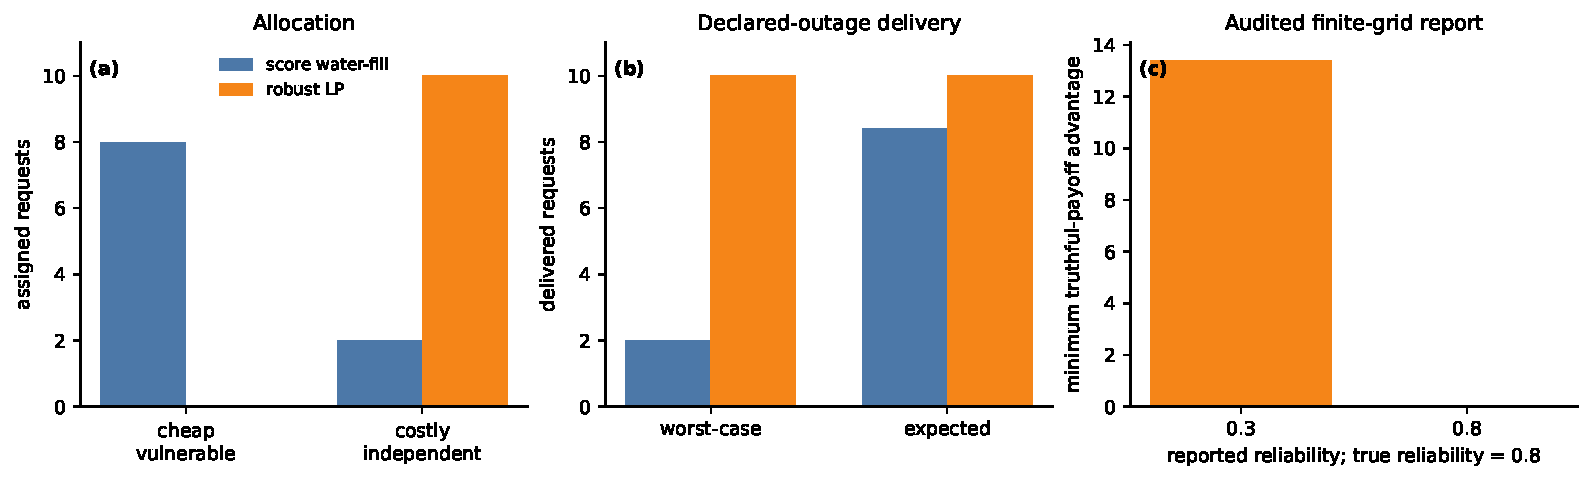
\includegraphics[width=\linewidth]{figures/synthetic_mechanism_examples.pdf}
\caption{Synthetic theorem illustrations generated by
\texttt{generate\_synthetic\_examples.py}. (a) The robust LP shifts
allocation away from a cheap provider exposed to a declared outage state.
(b) This raises the declared worst-case delivery floor while also improving
expected delivery in this particular instance. (c) The finite-grid score makes
the false reliability report strictly worse even after minimizing the
truthful-payoff advantage over the displayed capacity/cost deviations. No
panel is a measurement of a real provider.}
\label{fig:synthetic}
\end{figure}

\section{Hidden eligibility and a value-indexed routing experiment}
\label{sec:experiment}

The separation result in \cref{thm:separation} is a worst-case statement. We
next give an experiment that measures the value of information hidden behind a
router without claiming to observe that information. Let $\mathcal P$ be a
finite set of routing policies containing delegated default routing $d$ and
provider-pinned policies. In block $b$, let $S_b(p;h)\in\{0,1\}$ and
$C_b(p;h)\geq0$ denote success and observed billed cost when policy $p$ is run
after within-block history $h$. These are request outcomes, not provider costs.

Draw a random permutation of $\mathcal P$ independently in each block. Write
$P_b$ for the first policy and $\pi_{bp}=\Pr(P_b=p)>0$. The first request has
empty history. We require non-anticipation---its potential outcome does not
depend on policies that have not yet run---but impose no restriction on the
effect of the first request on later requests.

\begin{theorem}[First-position identification under post-request interference]
\label{thm:firstposition}
Conditional on the finite collection of first-exposure potential outcomes, the
Horvitz--Thompson estimators
\[
 \widehat\mu_S(p)=\frac1B\sum_{b=1}^B
 \frac{\mathbf 1\{P_b=p\}S_b^{\mathrm{obs}}}{\pi_{bp}},\qquad
 \widehat\mu_C(p)=\frac1B\sum_{b=1}^B
 \frac{\mathbf 1\{P_b=p\}C_b^{\mathrm{obs}}}{\pi_{bp}}
\]
are unbiased for $B^{-1}\sum_b S_b(p;\varnothing)$ and
$B^{-1}\sum_b C_b(p;\varnothing)$. Hence their policy differences identify
first-exposure success and observed-spend effects even if any request changes
every later potential outcome in its block.
\end{theorem}

The theorem is deliberately about the first position. A conventional
full-block crossover comparison additionally assumes away, models, or bounds
carryover. This matters when the likely failure is HTTP 429: sending one probe
can change the account-specific state faced by the next probe. Random order
turns later positions into a carryover diagnostic rather than silently treating
them as independent observations.

Let $\Delta S_p=\mu_S(d)-\mu_S(p)$ and
$\Delta C_p=\mu_C(d)-\mu_C(p)$. If a successful response has value $v\geq0$,
the observable policy-utility contrast is
\begin{equation}
\label{eq:valuefrontier}
 \Delta U_p(v)=v\Delta S_p-\Delta C_p.
\end{equation}

\begin{proposition}[Value frontier and delegation rescue]
\label{prop:valuefrontier}
If $\Delta S_p>0$, delegated routing is preferred under the request-level
value-minus-observed-spend criterion exactly when
$v>v_p^*=\Delta C_p/\Delta S_p$. If $\Delta C_p\leq0$, it weakly dominates for
every $v\geq0$. Moreover,
\[
 \Delta S_p=\Pr(S(d)=1,S(p)=0)-\Pr(S(d)=0,S(p)=1).
\]
Thus a positive success effect lower-bounds the frequency with which delegation
rescues a pinned failure; under monotone delegation, it equals that frequency.
\end{proposition}

The default-versus-pinned contrast is itself a composite treatment. Let $n$
pin the cheapest public provider with no fallback, let $f$ submit the full
public cheapest-first provider order with fallback, and let $d$ delegate both
selection and fallback to the router. Define
\[
 \Delta_F=\mu_S(f)-\mu_S(n),\qquad
 \Delta_I=\mu_S(d)-\mu_S(f),\qquad
 \Delta_T=\mu_S(d)-\mu_S(n).
\]

\begin{proposition}[Fallback-selection decomposition and non-identification]
\label{prop:decomposition}
The total delegation effect obeys $\Delta_T=\Delta_F+\Delta_I$. A randomized
comparison observing only $d$ and $n$ identifies $\Delta_T$ but not its two
components. In particular, even under the monotonicity restrictions
$\mu_S(d)\geq\mu_S(f)\geq\mu_S(n)$, every decomposition
$(\Delta_F,\Delta_I)=(a,\Delta_T-a)$ with
$a\in[0,\Delta_T]$ is observationally equivalent. Random assignment among
$d,f,n$ identifies both components from first-position outcomes under the
conditions of \cref{thm:firstposition}.
\end{proposition}

The proposition changes the interpretation of the experiment. $\Delta_F$ is
the option value of continuing past the same cheapest first provider under a
publicly reproducible order. $\Delta_I$ is the incremental value of replacing
that order with the router's delegated policy while preserving fallback
permission. It may reflect private eligibility, performance scores, contracts,
or other undocumented state; the experiment does not identify which signal the
router uses. The separately preregistered H81 study randomizes these three
policies on ranked models five and six, leaving the H80 four-arm holdout and its
stopping rule unchanged.

Equation \eqref{eq:valuefrontier} is a partial welfare object. It avoids choosing
a user value by reporting the full frontier, but it omits output-quality
differences, provider production cost, router transfers, and externalities.
Those omissions prevent a market-wide welfare interpretation.

\section{Measurement contract and empirical role}

Public provider listings can support descriptive quote and operational
heterogeneity, not the premises of the theorems. The companion RouteScope
protocol separates public quotes (L0), documented-policy simulations (L1),
public operational signals (L2), redacted selected-provider outcomes (L3), and
commitment/capacity outcomes (L4).

\begin{table}[t]
\centering
\footnotesize
\begin{tabular}{p{0.20\linewidth}p{0.32\linewidth}p{0.34\linewidth}}
\toprule
Model object & Current measurement status & Permitted use in this paper \\
\midrule
Posted quote $p_i$ & public quote for a fixed workload & score input and quote heterogeneity \\
Public performance & exact-match uptime and p90 fields are partial & coverage and missingness audit only \\
Simulated share $\hat s_i$ & documented public price proxy & mechanical comparative static only \\
Selection / retries & 616 owned attempts; 534 selected-provider fields & account/workload policy calibration only \\
Capacity / cost / value & no controlled commitment panel & theorem primitives and protocol fields only \\
Joint outage support & no joint-outage observations & declared synthetic support only \\
\bottomrule
\end{tabular}
\caption{The empirical boundary is part of the mechanism claim.}
\label{tab:empiricalboundary}
\end{table}

\Needspace{14\baselineskip}
The public quote simulation uses an inverse-square price rule only as an
exposed-policy calibration:
\[
  \hat s_i=\frac{q_i^{-2}}{\sum_jq_j^{-2}},\qquad
  \frac{\partial\log\hat s_i}{\partial\log q_i}=-2(1-\hat s_i).
\]
This derivative is mechanical, not an estimate of demand elasticity. It must
not be used as evidence of actual allocation, adverse selection, or
MEV-like behavior.

\subsection{Brown--MacKay pricing-technology screen}

The public quote panel also tests the pricing-technology channel emphasized by
Brown and MacKay \cite{brownmackay2023}. Across 2,062,359 endpoint snapshots in
1,684 capture runs, the retained completion-price event panel contains 274
changes over 7.53 days. Of 69 providers with sufficient quote exposure, only
19 reprice at all: 10 are classified intraday, six daily, and three weekly.
This supports heterogeneous pricing cadence but leaves most providers in a
no-observed-change group.

The stronger reaction-rule implication is not supported. In 115 independent
rival price waves, only 15 fast-provider windows follow a slow-provider move.
Their post-move response rate is 6.7\%, versus a 13.3\% pre-period placebo,
for a $-6.7$ percentage-point difference with a cluster interval of
$[-20.0,0.0]$ pp. A cadence-only regression finds that slow providers quote a
10.1\% premium over fast providers conditional on model, but state-based and
strategic reaction models trade off predictive metrics and the joint
competitive-null gate fails. We therefore use pricing technology as a
descriptive market characteristic, not evidence of algorithmic reaction,
collusion, or Brown--MacKay equilibrium effects.

\subsection{Randomized micro-probe protocol}

The fixed-order pilot sent four near-simultaneous one-token requests per hot
model: default routing, the cheapest displayed provider, the second-cheapest,
and a random remaining displayed provider. Pinned policies disabled fallback.
The prospective v2 collector uniformly permutes all four policies, publishes a
block identifier, seed, position, and first-position assignment probability,
and uses only position zero for the primary contrast. The protocol was frozen
after inspecting v1 and before collecting v2. Its first confirmatory cut
requires at least 40 first-position assignments per policy and 160 valid
blocks; HTTP and network failures remain intention-to-treat outcomes.

\begin{table}[t]
\centering
\small
\begin{tabular}{lrrrr}
\toprule
Policy & Attempts & Success & Wilson 95\% CI & HTTP 429 \\
\midrule
Default router & 96 & 97.9\% & [92.7, 99.4]\% & 1.0\% \\
Pinned cheapest & 96 & 80.2\% & [71.1, 86.9]\% & 18.8\% \\
Pinned second & 96 & 66.7\% & [56.8, 75.3]\% & 33.3\% \\
Pinned random & 96 & 76.0\% & [66.6, 83.5]\% & 21.9\% \\
\bottomrule
\end{tabular}
\caption{Matched v1 pilot outcomes. Every default request preceded the pinned
arms, so intervals describe marginal rates and do not remove the policy/order
confound.}
\label{tab:pilot}
\end{table}

\begin{figure}[t]
\centering
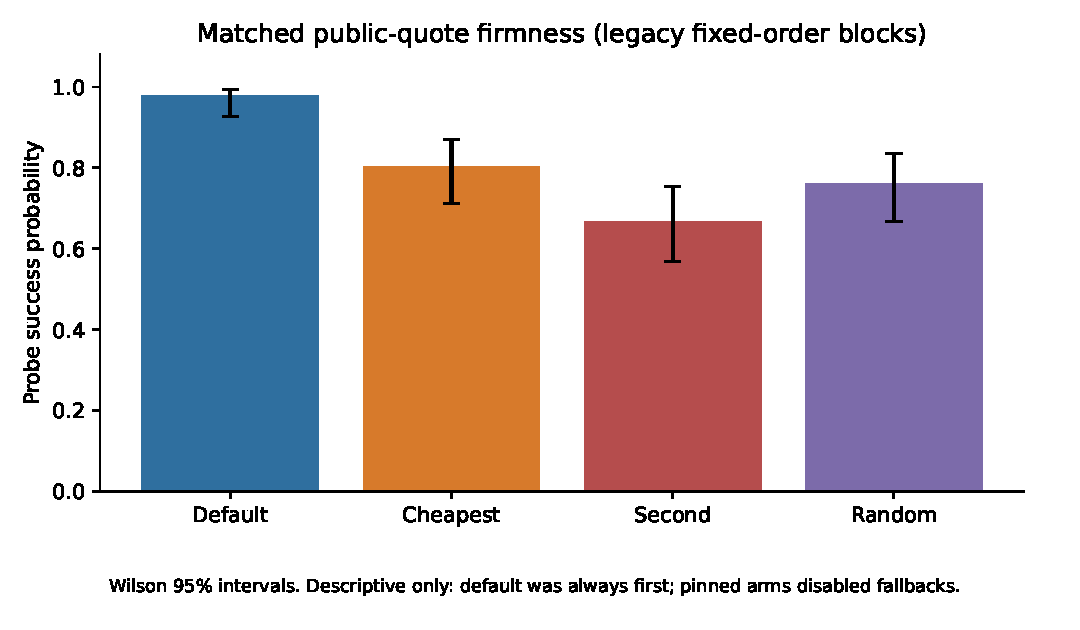
\includegraphics[width=0.82\linewidth]{../../analysis/h80_quote_firmness.pdf}
\caption{Matched public-quote firmness in the 24-hour v1 pilot. Error bars are
Wilson intervals for policy-specific success rates. The prospective v2
first-position analysis, not this figure, supplies the causal contrast.}
\label{fig:firmness}
\end{figure}

\subsection{A falsifiable mechanism implementation study}

A mechanism implementation study must pre-register model-by-epoch policy
assignment, commitments, served count, fallback cost, a value-minus-cost proxy,
and a latency negative control. The primary estimands are:
\begin{enumerate}
  \item the selected-provider and fallback calibration of pre-request public
  features;
  \item the delivery-floor and shortfall difference between capacity-certified
  and baseline routing under observed commitments;
  \item the funded-contract accounting residual under the two polar states in
  \cref{eq:treasury}; and
  \item a declared value-net-cost proxy, only when its value and cost inputs are
  retained and versioned.
\end{enumerate}
Each item has a failure mode. A public shadow can fail to predict selection
because live eligibility is hidden. The robust program can fail to improve
delivered count if the declared outage support is misspecified. A collateral
certificate can be infeasible because a provider cannot fund the required
collateral. A welfare claim fails closed whenever request value, delivery cost,
or capacity outcome is missing. These are not caveats added after estimation;
they are preconditions for interpreting the mechanism.

\subsection{Current evidence}

The v1 pilot contains 96 complete blocks across four models and 23 hourly
common-shock clusters over 24 hours; the median block span is 29.5 seconds.
Default routing succeeded 17.7 percentage points more often than the cheapest
displayed provider (hour-cluster bootstrap 95\% CI 9.2--26.4 pp; cluster
sign-flip $p=0.0019$), 31.3 pp more often than second-cheapest (24.4--38.0 pp),
and 21.9 pp more often than random (16.7--27.2 pp). Default selected the
displayed cheapest provider in only 21 of 96 blocks and selected a provider
outside the three sampled pinned identities in 45 blocks.

For cheapest versus default, the observed-spend difference in the 94 blocks
with complete accounting and the 96-block success difference imply
$v^*=2.13\times10^{-5}$ dollars per successful request in the pilot. This is a
complete-accounting descriptive threshold, not a willingness-to-pay estimate.
Most importantly, default was first in every block and pinned requests disabled
fallback. The pilot therefore establishes a matched quote-firmness gap for this
account and workload, not a causal delegation effect. The preregistered v2
first-position sample is the prospective test.

\section{Limitations and conclusion}

The mechanism requires more information than a public marketplace currently
reveals: verified or collateralized capacity, collectable liability, a finite
report domain, independently assigned objective audits, an external audit fund,
and a declared joint-outage support. The owned probes identify neither those
private inputs nor provider intent, other users' flow, or literal front-running.
The current pilot also confounds policy and order. These limitations are the
result: displayed prices alone do not supply a delivery guarantee, and the
value of hidden eligibility requires a prospective experiment rather than a
retrospective causal label.

\bibliographystyle{plain}
\bibliography{../references}

\appendix
\section{Proofs}

\subsection{Proof of the capped allocation theorem}
Let
\[
 F=\{x\geq0:\sum_i x_i=D,\ x_i\leq k_i\}.
\]
The set is nonempty exactly when $D\leq\sum_i k_i$, compact, and convex. The
objective in \cref{eq:primal} is strictly concave on each positive-dimensional
feasible face. Its derivative from zero is positive whenever an uncapped
positive-weight coordinate is available, so the allocation maximizer is
unique. KKT stationarity on an uncapped coordinate gives
$\log w_i-\log x_i-1=\lambda$, hence $x_i=\tau w_i$. Complementary slackness
gives the cap. The function
$\sum_i\min\{k_i,\tau w_i\}$ is continuous and nondecreasing from zero to
$\sum_i k_i$, so it reaches $D$. If every coordinate caps, the allocation is
still unique even though $\tau$ need not be.

\subsection{Proofs of delivery and delivered-count results}
Delivery yields $p_i-c_i$; deliberate refusal yields
$-\min\{b_i,L_i\}$. Their difference proves \cref{thm:delivery}. For
\cref{thm:count}, the capped allocation sums to $D$ and every assigned unit is
delivered by assumption. Under the uncapped rule, provider $i$ can deliver at
most $\min\{Ds_i,k_i\}$, and summing gives the result.

\subsection{Proof of the price-only separation}
Fix a public profile $(p_i,q_i)$ and a provider receiving a positive
allocation. Two capacity states are observationally equivalent to the rule:
one has enough capacity to serve its allocation; the other has zero capacity.
The rule makes the same assignment in both states, while delivery is impossible
in the second. Without delivery observation or enforcement, the rule cannot
repair that failure from $(p_i,q_i)$ alone.

\subsection{Proof of first-position identification and the value frontier}
Condition on all first-exposure potential outcomes. Random assignment gives
\[
 \E\left[\frac{\mathbf 1\{P_b=p\}S_b^{\mathrm{obs}}}{\pi_{bp}}\right]
 =\frac{\pi_{bp}S_b(p;\varnothing)}{\pi_{bp}}
 =S_b(p;\varnothing),
\]
where non-anticipation lets the observed first-position outcome equal the
corresponding empty-history potential outcome. Summing over blocks and dividing
by $B$ proves the success claim; the cost claim is identical. No outcome after
the first position appears in the estimator, so its dependence on earlier
requests is unrestricted.

For a policy $p$, expected value-minus-observed-spend is
$v\mu_S(p)-\mu_C(p)$. Subtracting pinned from delegated policy gives
\cref{eq:valuefrontier}. When $\Delta S_p>0$, division by $\Delta S_p$ gives
the threshold; if also $\Delta C_p\leq0$, the difference is nonnegative for
every $v\geq0$. Finally, partition the binary pair $(S(d),S(p))$ into its four
possible values. The equal pairs cancel from
$\E[S(d)-S(p)]$, leaving rescue probability minus harm probability. Rescue
probability is therefore at least $\max\{\Delta S_p,0\}$, and monotonicity
sets the harm term to zero.

For \cref{prop:decomposition}, add and subtract $\mu_S(f)$ in $\Delta_T$.
If only $\mu_S(d)$ and $\mu_S(n)$ are observed, choose any
$a\in[0,\Delta_T]$ and set $\mu_S(f)=\mu_S(n)+a$. This intermediate mean lies
between the observed endpoint means and produces
$(\Delta_F,\Delta_I)=(a,\Delta_T-a)$ without changing the distribution of
either observed arm. Randomizing the intermediate policy makes $\mu_S(f)$ an
identified first-position mean by \cref{thm:firstposition}, so subtraction
identifies both components.

\Needspace{14\baselineskip}
\subsection{Proof of robust delivery-floor dominance}
The feasible set of \cref{eq:robust} is nonempty because $x=0,z=0$ is feasible,
and it is compact because demand and every capacity cap bound the variables.
Take the capacity-feasible score allocation $x^S$ and set
\[
 z^S=\min_{\omega\in\Omega^+}\sum_i a_i(\omega)x_i^S.
\]
Then $(x^S,z^S)$ is feasible for \cref{eq:robust}. Optimality of $(x^R,z^R)$
therefore gives $z^R\geq z^S$, which is the claimed inequality. A secondary
score objective ranges only over allocations with $z=z^R$, so it cannot lower
the floor. If a support state has $a_i(\omega)=0$ for all $i$, every feasible
allocation has delivered count zero in that state, proving
\cref{prop:commonmode}.

\subsection{Proof of the finite-liability boundary}
At true reliability $q$, expected payoff per assigned request is
$qm-(1-q)\ell$. Multiplying by the allocation increment
$x(r)-x(q)$ gives the displayed gain. The bracket is positive exactly when
$q>\ell/(m+\ell)$.

\subsection{Proof of collateralized finite-slot VCG}
Fix reliability reports. Let $W_{-i}^*$ be the maximum reported surplus
without provider $i$, including the outside option, and let $W_{-i}(x)$ be the
other-participant plus outside-option surplus under allocation $x$. The pivot
payment equals the provider's reported own buyer value plus
$W_{-i}(x)-W_{-i}^*$. For a true type $t_i$ and report $\hat t_i$, expected
utility before the audit is a report-independent constant plus the total
surplus evaluated with $t_i$ at the allocation selected by $\hat t_i$.
Truthfully reporting $t_i$ selects an allocation that maximizes that true
surplus, so no capacity/cost report can improve utility. The opt-out allocation
is feasible; removing a provider weakly restricts achievable surplus, which
gives nonnegative truthful utility. A false unavailable slot is included in
the true cost at $H>v$, so it cannot evade this comparison.

\subsection{Proof of the audited finite-grid construction}
Hold reliability reports fixed. The preceding pivot argument makes the true
capacity/cost type weakly optimal conditional on those reports. For an audit
outcome,
\[
 \E_q[S_A(q,Y)-S_A(r,Y)]
 =A\KL(\mathrm{Bern}(q)\Vert\mathrm{Bern}(r)).
\]
Because an audit occurs with probability $\rho$, the expected score advantage
is $\rho A$ times this quantity. Conditional VCG truthfulness bounds the
utility from any joint report $(\hat t_i,r)$ by the utility from $(t_i,r)$.
When $r\ne q$, \cref{eq:scale} makes the score advantage exceed the largest
remaining VCG gain by $\delta$. A deviation retaining $r=q$ is weakly
unprofitable by VCG. The opt-out allocation gives nonnegative VCG utility, and
the shifted score is nonnegative, proving individual rationality.

\end{document}
